\documentclass{article}
\usepackage{graphicx} % Required for inserting images
\usepackage[top=0.9in, bottom=1in, left=1.0in, right=1.0in]{geometry}
\usepackage[utf8]{inputenc}
\usepackage[icelandic]{babel}
\usepackage[T1]{fontenc}
\usepackage[sc]{mathpazo}
\usepackage[parfill]{parskip}
\renewcommand{\baselinestretch}{1.2}
\usepackage{booktabs,tabularx}
\usepackage{multirow}
\usepackage{enumerate}
\usepackage{adjustbox}
\usepackage{multicol}
\usepackage{xcolor}
\usepackage{algpseudocode}
\usepackage{tikz}
\usepackage{nicefrac}
\usepackage{changepage}
\usetikzlibrary{arrows, positioning, calc, graphs}
\usepackage{amsmath, amsfonts, amssymb, amsthm}
\usepackage{graphicx}
\usepackage{tikz}
\usepackage{minted}
\usemintedstyle{manni}
\title{Tölvutækni og Forritun Verkefni 2}
\author{Ragnar Björn Ingvarsson, rbi3 \\
        Yi Hu, yih2}
\tikzset{->, >=stealth', shorten >=1pt, node distance=2cm,thick, main node/.style={circle,draw,minimum size=3em}}

\begin{document}
\renewcommand\thepage{}

	\maketitle

	\newpage
	\setcounter{page}{1}
	\renewcommand\thepage{\arabic{page}}
	\renewcommand\thesection{\Roman{section}}
	\renewcommand\thesubsection{\Roman{section}.\roman{subsection}}

	\section{Skrifa hermi fyrir skyndiminni}
	\begin{minted}{c}
void initCache()
{
    cache = (cache_set_t*) malloc(S*sizeof(cache_set_t));
	for (int i = 0; i < S; i++) {
		cache[i] = (cache_line_t*) malloc(E*sizeof(cache_line_t));
	}
}

void freeCache()
{
	free(cache);
}

void accessData(mem_addr_t addr)
{
	long set = (addr >> b) & ((1ULL << s) - 1);
	long tag = addr >> (s+b);

	int has_hit = 0;
	int insert_place = -1;
	int lowest_value = policy_code == 1 ? cache[set][0].lru : cache[set][0].fifo;
	int lowest_index = 0;

	for (int i = 0; i < E; i++) {

		cache_line_t line = cache[set][i];

		if (policy_code == 1) {
			if (lowest_value > line.lru) {
				lowest_value = line.lru;
				lowest_index = i;
			}
		} else if (policy_code == 2) {
			if (lowest_value > line.fifo) {
				lowest_value = line.fifo;
				lowest_index = i;
			}
		}

		if (line.valid && line.tag == tag) {
			line.lru = ++lru_counter;
			hit_count++;
			has_hit = 1;
			cache[set][i] = line;
			break;
		}
		if (!line.valid) {
			insert_place = i;
		}
	}
	if (!has_hit) {
		miss_count++;
		if (insert_place == -1) {
			insert_place = policy_code == 3 ? rand() % E : lowest_index;
			eviction_count++;
		}
		cache_line_t line_to_be_added;
		line_to_be_added.tag = tag;
		line_to_be_added.fifo = fifo_counter++;
		line_to_be_added.lru = lru_counter++;
		line_to_be_added.valid = 1;
		cache[set][insert_place] = line_to_be_added;
	}
}
	\end{minted}

	\vspace{6em}

	\begin{center}
		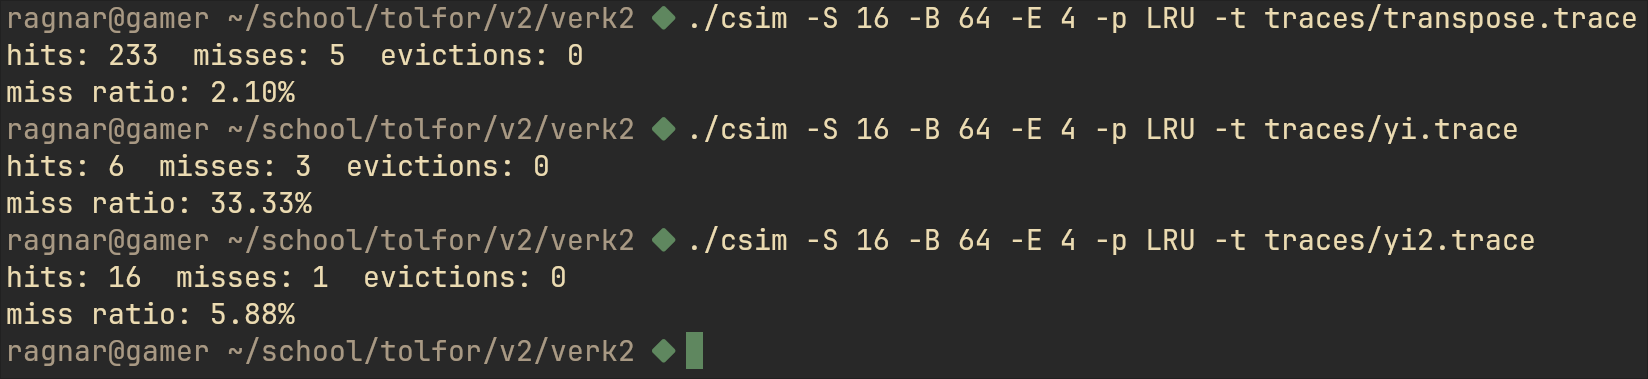
\includegraphics[width=0.95\textwidth]{result.png}
	\end{center}

	\newpage
	\section{Besta uppsetning á skyndiminni}
	\begin{multicols}{2}
	\begin{figure}[H]
		\begin{center}
			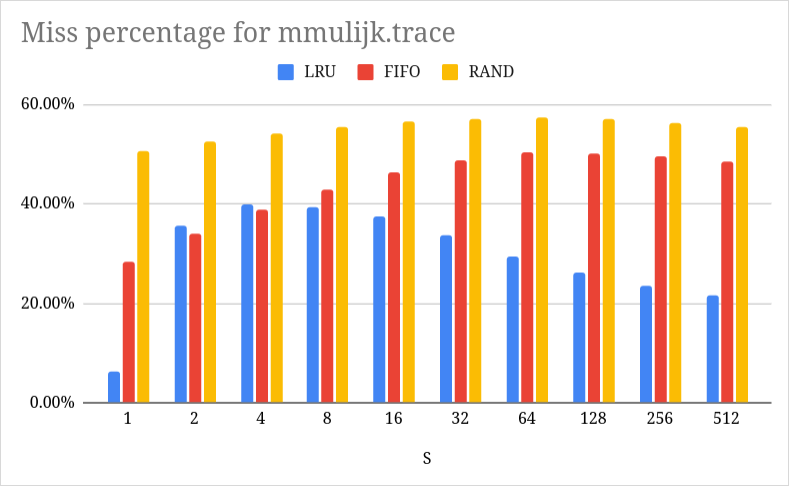
\includegraphics[width=0.48\textwidth]{mmul.png}
		\end{center}
		\caption{\texttt{mmulijk.trace}}\label{fig:mmul}
	\end{figure}
	\begin{figure}[H]
		\begin{center}
			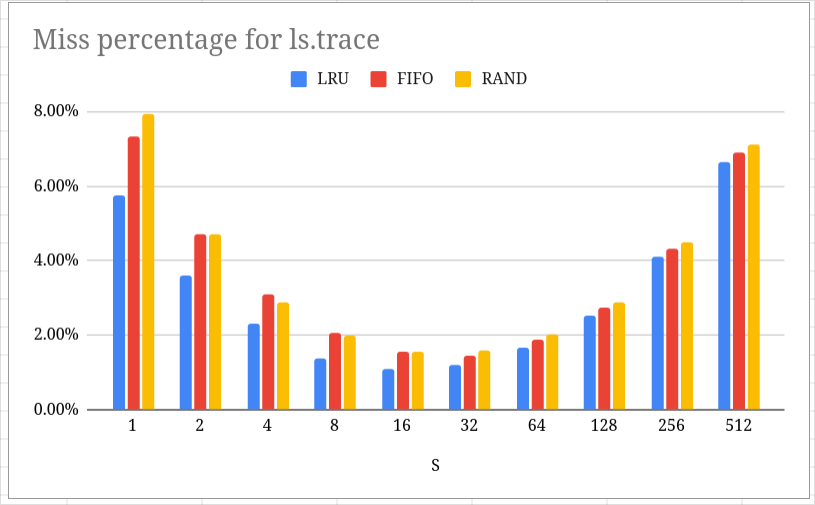
\includegraphics[width=0.48\textwidth]{ls.png}
		\end{center}
		\caption{\texttt{ls.trace}}\label{fig:ls}
	\end{figure}
	\end{multicols}
	
	\subsection{Hver er munurinn á bestu uppsetningu á milli 
	rakningaskránna?}
	Við sjáum af súluritunum að það er töluverður munur á keyrslu milli 
	rakningaskránna. Fyrir \\ \texttt{mmulijk.trace} kemur langverst út að 
	hafa $S$ mjög lítið, en svo er langbest að hafa það einhversstaðar 
	í miðjunni um $16$-$32$, þar sem það virðist ekki vera betra að vera 
	með of mörg mengi. 

	Með \texttt{ls.trace} þá sést að það myndast dalur í 
	ritinu, svo það er best sð vera aftur, í kring um $16$-$32$. 

	Munurinn hér er væntanlega vegna þess að þar sem \texttt{ls.trace} 
	er mjög óreglulegt og út um allt, þá er best að setja upp minnið okkar 
	þannig að við séum með jafnan fjölda mengja og stærð línanna, þar sem 
	ef við förum of langt í aðra hvora áttina þurfum við að leita svo djúpt
	í staðinn fyrir að leita grunnt á báða ása. Þetta hjálpar að mynda eins 
	mikið "bil" á milli gagnanna svo við lendum ekki í skellum.

	\texttt{mmulijk.trace} er hins vegar mjög reglulegt og þess vegna 
	viljum við notfæra okkur að gögnin eru alltaf hlið við hlið. Þess vegna 
	er svo mikilvægt að hafa ekki of stórar línur því þá flækjast gögn 
	kannski saman í línur og valda fleiri skellum, svo við viljum 
	hafa nógu litlar línur til að bara halda utan um gögnin sem við erum 
	nú þegar að vinna með en nógu stórar svo við séum heldur ekki að 
	henda út gögnum sem við erum að nota. 

	Svo besta uppsetningin fyrir \texttt{mmulijk} er $S=32$ á $LRU$ og 
	fyrir \texttt{ls} er $S=16$ á $LRU$.

	\subsection{Hvernig kemur uppsetning Intel Core i7 út í hermunum?}
	Við sjáum að þetta er sama uppsetningin og við vorum að prófa og það 
	sést á súluritunum að þetta er ekki besta uppsetningin hvorki fyrir 
	\texttt{mmulijk.trace} né \texttt{ls.trace} en hún er samt alls ekki 
	sú versta og kemur bara mjög vel út í báðum tilfellum. 

	Ég myndi þá halda að ástæðan fyrir að velja svona uppsetningu sé 
	vegna þess að hún sé kannski best ef við prófum yfir fleiri tilfelli 
	af rakningaskrám og líka að það sé kannski betra fyrir orkusparnað 
	eða pláss eða kostnað og svoleiðis. 
	
\end{document}
